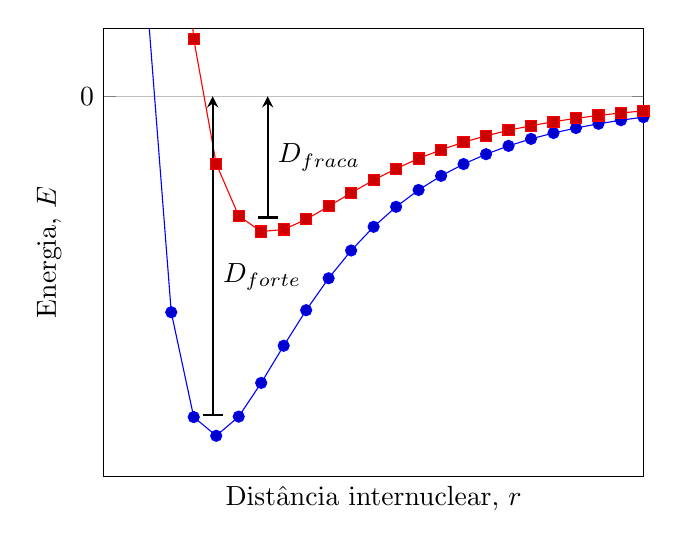
\begin{tikzpicture}
\begin{axis}
    [
        grid = major,
        ylabel = {Energia, $E$},
        xlabel = {Distância internuclear, $r$},
        domain = 0.9:2,
        xmin = 0.9, xmax = 2,
        ymax = 2,
        xtick=\empty, ytick=0,
    ]
\addplot
    {
        4 * 10 * ((1/x)^(12) - (1/x)^6)
    };
    \addplot
    {
        4 * 4 * ((1.1/x)^(12) - (1.1/x)^6)
    };
    \draw [ draw=black, thick, |-stealth ]
        (axis cs: 1.122, -9.4) -- node [right, align=center] { \\[1em] $D_\text{forte}$}
        (axis cs: 1.122, -0);
    \draw [ draw=black, thick, |-stealth ]
        (axis cs: 1.234, -3.6) -- node [right] {$D_\text{fraca}$}
        (axis cs: 1.234, -0);
\end{axis}
\end{tikzpicture}

\end{document}
